\documentclass[]{article}

\usepackage{tikz}
\usepackage{lipsum}  % For generating dummy text

%opening
\title{}
\author{}

\begin{document}

\maketitle

\begin{abstract}

\end{abstract}

\section{Diagram Examples}

\begin{tikzpicture}
	\draw (0,0) -- (4,0) -- (4,4) -- (0,4) -- cycle;
\end{tikzpicture}

\subsection{Squiggle}

\begin{tikzpicture}
	\draw (0,0) rectangle  (4,4);
\end{tikzpicture}

\subsection{Parabola}

\begin{tikzpicture}
	\draw (0,0) parabola  (-4,4);
\end{tikzpicture}

\subsection{Rectangle}

\begin{tikzpicture}
	\draw (0,0) .. controls (0,4) and (4,0) .. (4,4);
\end{tikzpicture}

\subsection{Circle}

\begin{tikzpicture}
	\draw (0,0) circle  (3cm);
\end{tikzpicture}

\subsection{Ellipse}

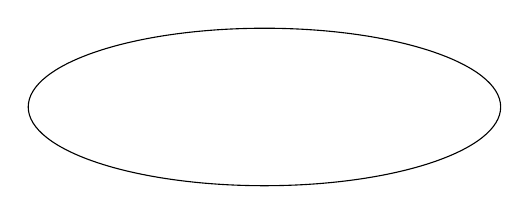
\begin{tikzpicture}
	\draw (0,0) ellipse  (3cm and 1cm);
\end{tikzpicture}

\subsection{Arc}

\begin{tikzpicture}
	\draw (0,0) arc  (0:75:3cm);
\end{tikzpicture}

\subsection{Circle}

\begin{tikzpicture}
	\draw[red,thick,dashed]  (2,2) circle  (3cm);
\end{tikzpicture}

\newpage


\subsection{Grids}

\subsubsection{Bounded Grid}

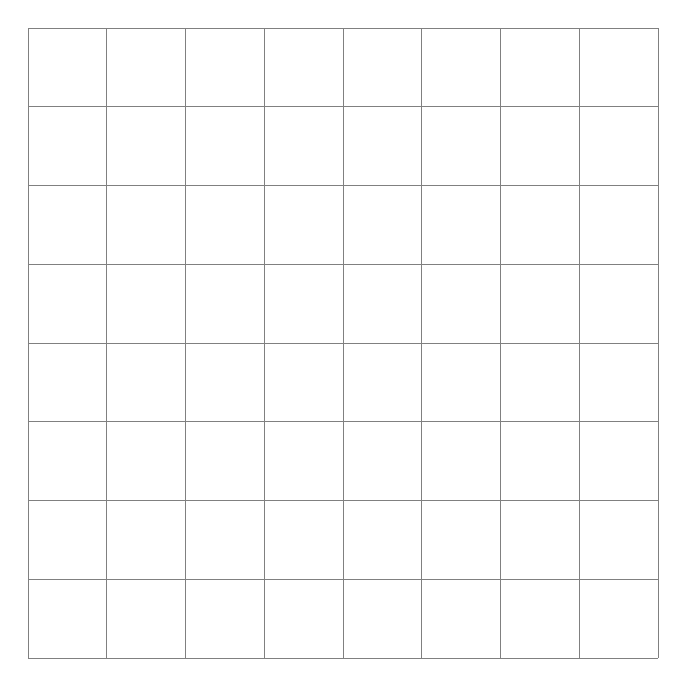
\begin{tikzpicture}
	\draw[step=1cm,gray,very thin]  (-2,-2) grid  (6,6);
\end{tikzpicture}

\subsubsection{Unbounded Grid - Very Thin}

\begin{tikzpicture}
	\draw[step=1cm,gray,very thin]  (-1.9,-1.9) grid  (5.9,5.9);
\end{tikzpicture}

\subsubsection{Unbounded Grid - Thin}

\begin{tikzpicture}
	\draw[step=1cm,gray,thin, dashed]  (-1.9,-1.9) grid  (5.9,5.9);
\end{tikzpicture}

\subsubsection{Unbounded Grid - Thick}

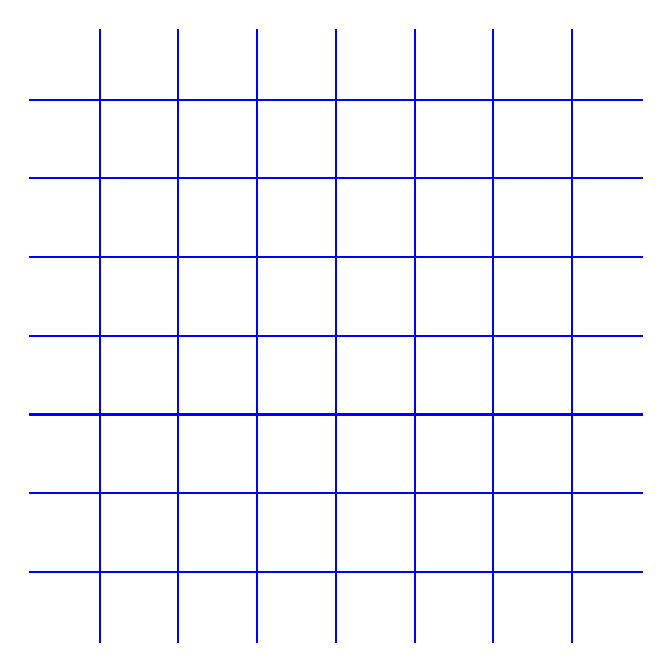
\begin{tikzpicture}
	\draw[step=1cm,blue,thick]  (-1.9,-1.9) grid  (5.9,5.9);
\end{tikzpicture}


\newpage


\end{document}
